\documentclass{standalone}
\usepackage[T1]{fontenc}
\usepackage{amsmath,amssymb}
\usepackage{pgfplots}

\begin{document}
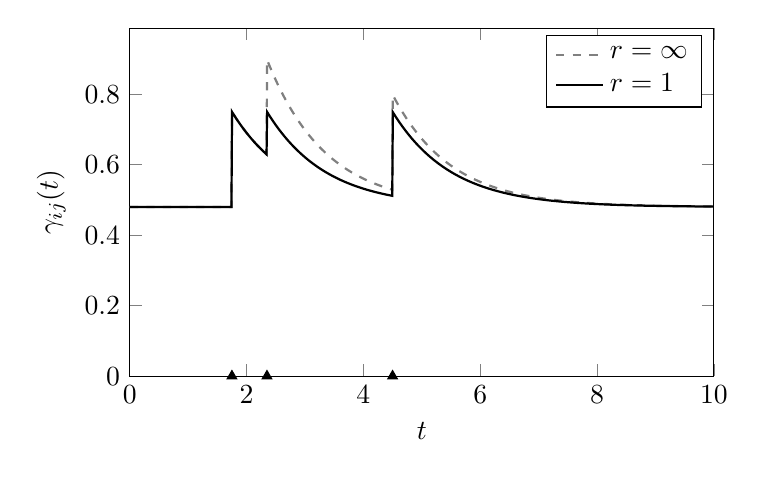
\begin{tikzpicture}
\begin{axis}[xmin=0,xmax=10,ymin=0,xlabel=$t$,ylabel=$\gamma_{ij}(t)$,height=6cm,width=9cm, legend cell align={left}]
	
	\def\inta{0.8}
	\def\intb{0.6}
	\def\shapa{0.9}
	\def\shapb{0.3}
	\def\scala{2.0}
	\def\scalb{0.5}
	
	\addplot[domain=0:10, samples=1000, style=thick, dashed, gray] {
	(\inta*\intb + 
	(x > 1.75 ? \shapa*\shapb*exp(-\scala*\scalb*(x-1.75)) : 0) + 
	(x > 2.35 ? \shapa*\shapb*exp(-\scala*\scalb*(x-2.35)) : 0) + 
	(x > 4.50 ? \shapa*\shapb*exp(-\scala*\scalb*(x-4.50)) : 0)
	)};
	\addlegendentry{$r=\infty$};

	\addplot[domain=0:10, samples=1000, style=thick] {
	(\inta*\intb + 
	(x > 1.75 ? \shapa*\shapb*exp(-\scala*\scalb*(x-1.75)) : 0) + 
	(x > 2.35 ? \shapa*\shapb*exp(-\scala*\scalb*(x-2.35))-\shapa*\shapb*exp(-\scala*\scalb*(x-1.75)) : 0) + 
	(x > 4.50 ? \shapa*\shapb*exp(-\scala*\scalb*(x-4.50))-\shapa*\shapb*exp(-\scala*\scalb*(x-2.35)) : 0)	
	)};
	\addlegendentry{$r=1$};
	
	\addplot[mark=triangle*] coordinates {(1.75,0)};
	\addplot[mark=triangle*] coordinates {(2.35,0)};
	\addplot[mark=triangle*] coordinates {(4.5,0)};

\end{axis}
\end{tikzpicture}
\end{document}
